% Copyright 2023 by Johan van der Molen Moris, 2015 by Paul Kirk
%
% This file may be distributed and/or modified
%
% 1. under the LaTeX Project Public License and/or
% 2. under GPLv3.

\documentclass[aspectratio=169, 12pt]{beamer} %we use these options to obtain the powerpoint aspect ratio and fontsize
\usetheme[pageofpages=of,% String used between the current page and the total page count.
  ]{BSU}

\usepackage{pgf,tikz}

\usepackage{graphicx}
\graphicspath{{./figs/}}
\usepackage{appendixnumberbeamer}

\author[]{Name Lastname}
\title[]{Presentation introduction}
\subtitle[]{Presentation introduction subheading}
\institute{MRC Biostatistics Unit}
\date{\today}

\begin{document}
%%%%%%%%%%%%%%%%%%%%%%%%%
%% Title frame 
%%
\begin{frame}[plain]
\titlepage
\setcounter{framenumber}{0}
\end{frame}
%%%%%%%%%%%%%%%%%%%%%%%%%
%

\begin{frame}[t]{Copy Only}
    % [t] option vertically aligns the text at the top
    % and it makes it look more like the PowerPoint template.
    % When removed the text is centred.
    Quisque sagittis purus sit amet volutpat consequat mauris nunc congue nisi vitae suscipit tellus \textbf{mauris} a diam maecenas sed enim ut sem viverra aliquet eget sit amet tellus cras adipiscing enim eu turpis egestas pretium aenean pharetra magna ac placerat vestibulum lectus mauris ultrices eros in cursus turpis massa tincidunt dui ut ornare lectus sit amet est placerat in egestas erat imperdiet sed euismod nisi porta lorem mollis \textbf{aliquam} ut porttitor leo a diam sollicitudin \textbf{tempor.}
\end{frame}

\begin{frame}[t]{Making your presentations accessible}
  \heading{General guidance}  
  \begin{itemize}
    \item use our primary font Arial for all presentation text
    \item font size should be at least 12-14 point
    \item avoid underlining and italics
    \item use \textbf{bold} for emphasis
    \item avoid writing in all capital letters or all small caps
  \end{itemize}
\end{frame}

\begin{frame}[t]{Making your presentations accessible}
    \heading{Headings}  
    \begin{itemize}
      \item use headings to help people navigate through your content
      \item for headings, use a font size that is at least 20\% larger than the normal text
      \item use \textbf{bold} for emphasis
      \item add extra space around headings and between paragraphs
      \item ensure \alert{\underline{\smash{hyperlinks}}} look different from headings and normal text
    \end{itemize}
  \end{frame}

  \begin{frame}[t]{Making your presentations accessible}
    \heading{Aligning text}  
    \begin{itemize}
      \item left align text, without justification
      \item avoid multiple columns (as used in newspapers)
      \item lines should not be too long: 60 to 70 characters
      \item use white space to group related content
    \end{itemize}
  \end{frame}

  \begin{frame}{Bar chart}
      \begin{minipage}[l]{0.47\textwidth}
        \raggedright
        Quisque sagittis purus sit amet volutpat consequat mauris nunc congue nisi vitae suscipit tellus mauris a diam maecenas sed enim ut sem viverra aliquet eget sit amet tellus cras adipiscing enim eu turpis egestas pretium aenean pharetra magna ac placerat vestibulum lectus mauris ultrices eros in cursus turpis massa tincidunt dui ut ornare lectus.
      \end{minipage}
      \hfill
      \begin{minipage}{0.5\textwidth}
        \centering
        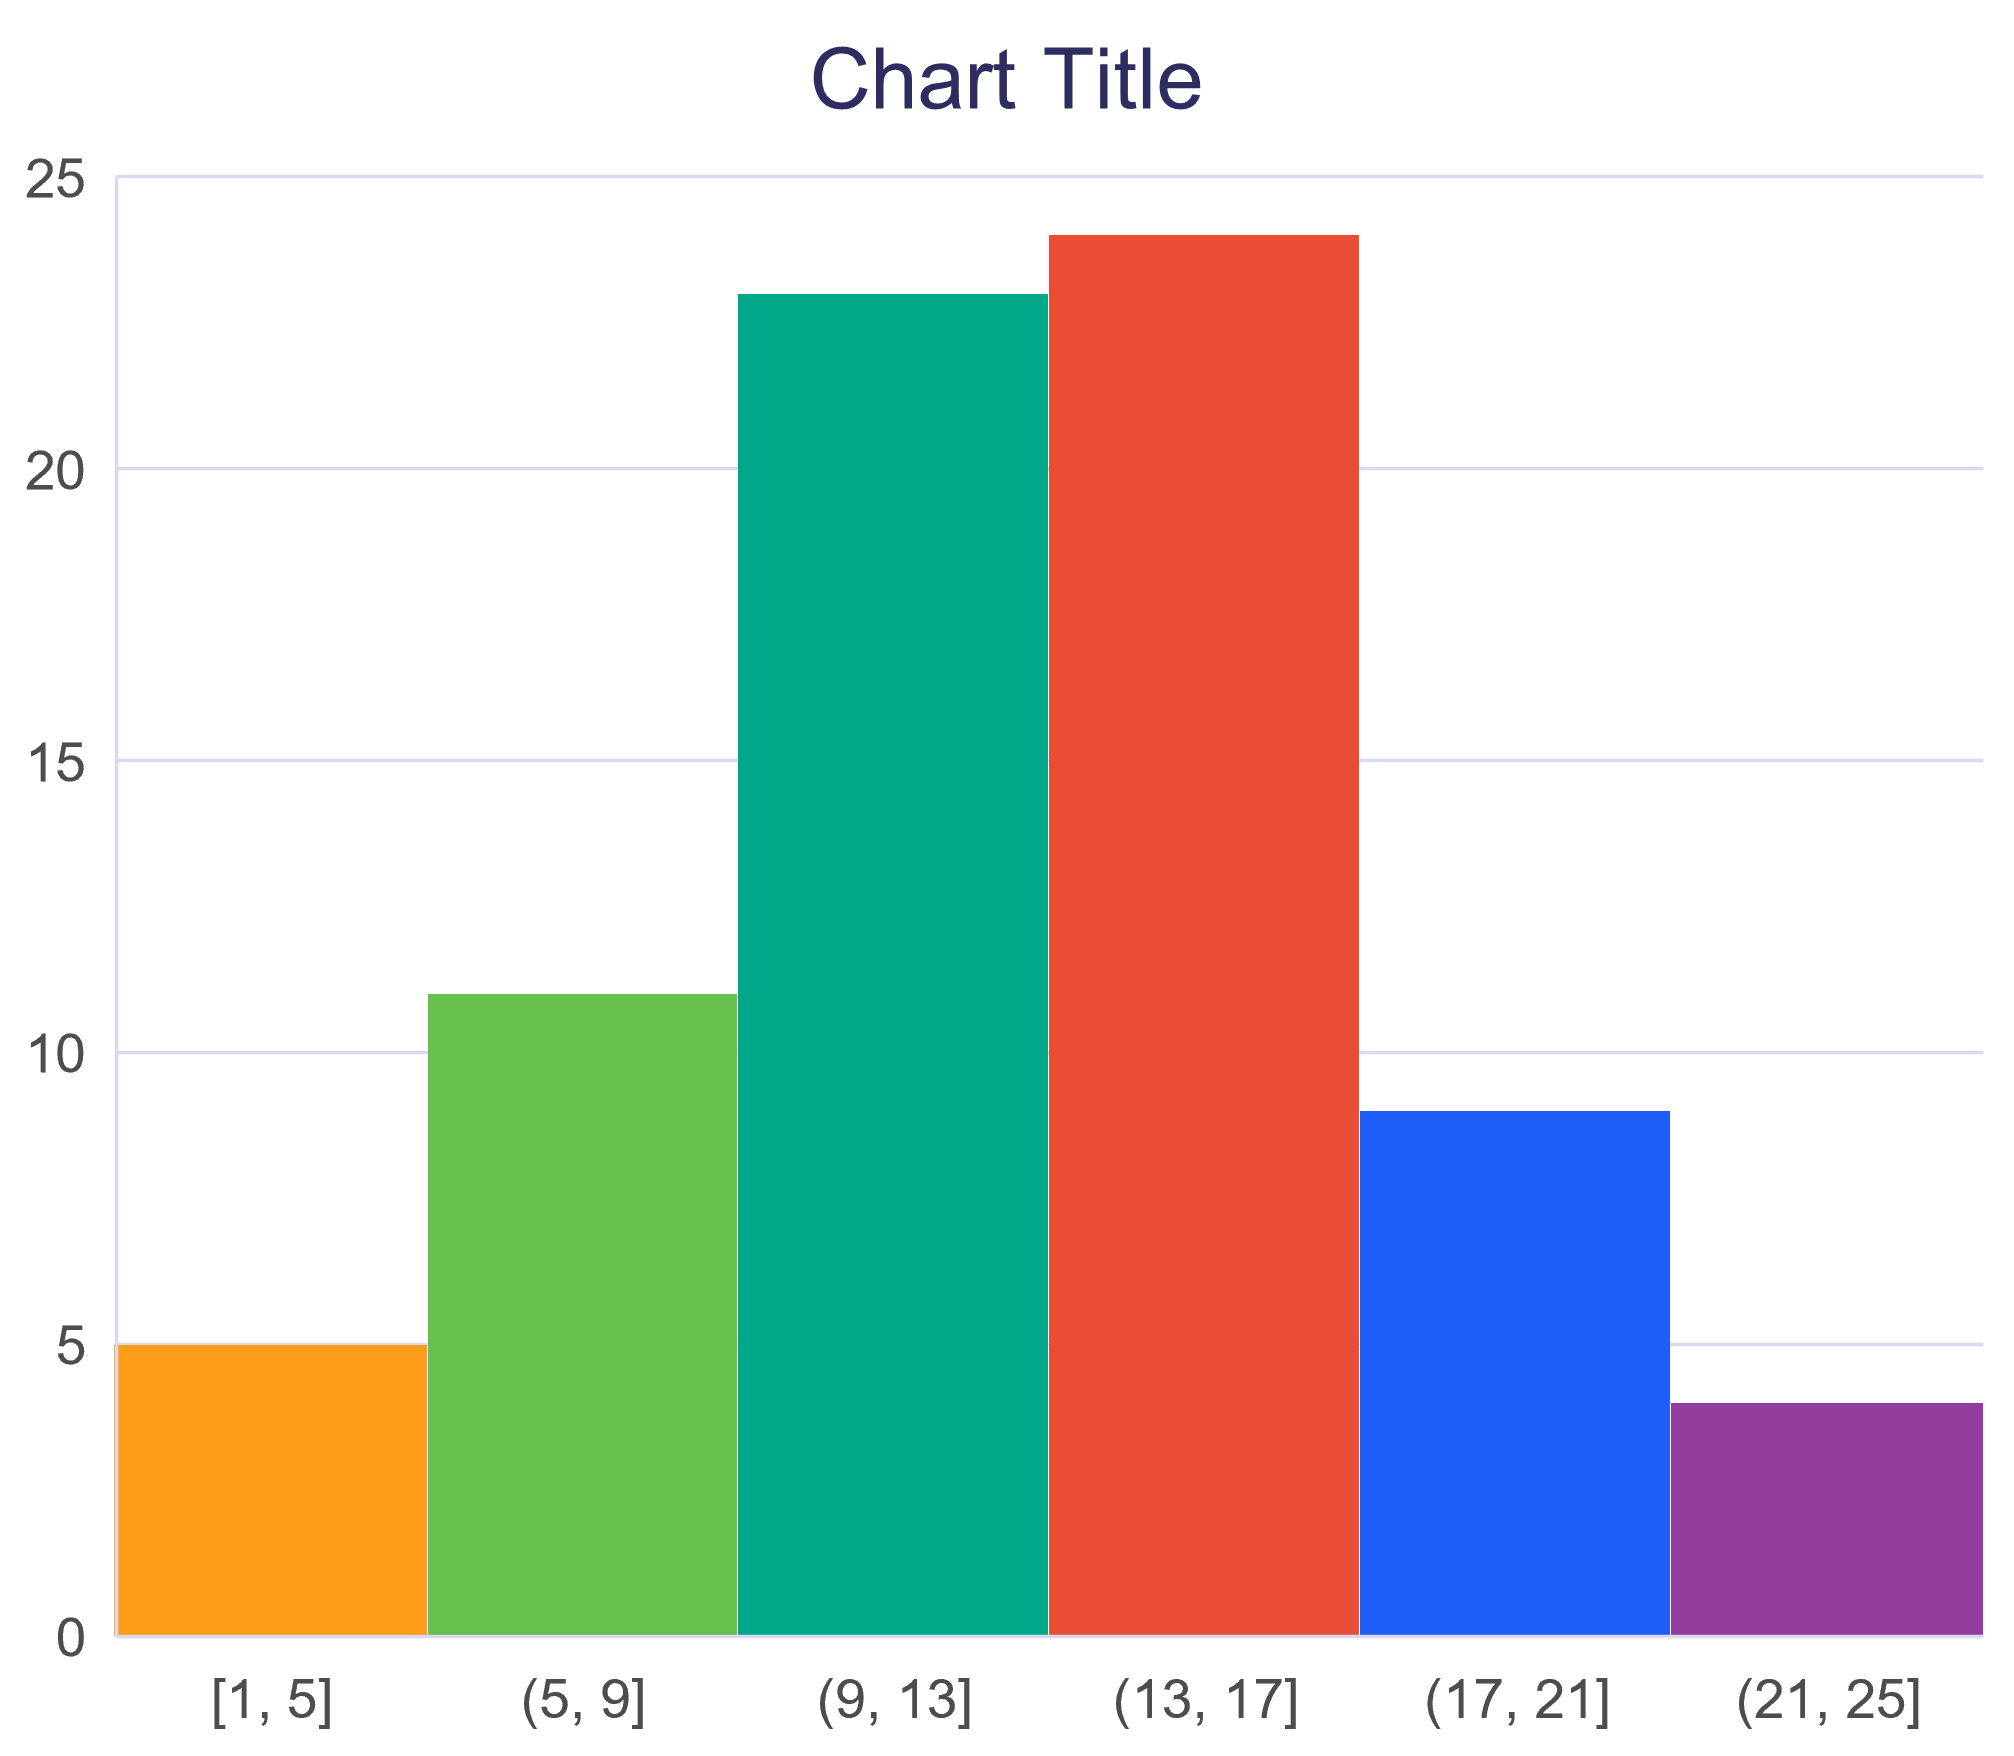
\includegraphics[width=\textwidth]{bar_chart}
      \end{minipage}
  \end{frame}

  \begin{frame}{Blocks}
    \begin{block}{Block}
      Quisque sagittis purus sit amet volutpat consequat mauris
    \end{block}

    \begin{exampleblock}{Example Block}
      Quisque sagittis purus sit amet volutpat consequat mauris
     
    \end{exampleblock}

    \begin{alertblock}{Alerted Block}
      Quisque sagittis purus sit amet volutpat consequat mauris      
    \end{alertblock}
  \end{frame}
  
  %the commands \questionspage and \thankyoupage inside a plain frame add
  %the questions and thank you slides from the template
  \begin{frame}[plain]
    \questionspage
  \end{frame}

  \begin{frame}[plain]
    \thankyoupage
  \end{frame}

\end{document}